%----------------------------------------------------------------------------------------
%	PACKAGES AND OTHER DOCUMENT CONFIGURATIONS
%----------------------------------------------------------------------------------------

\documentclass[
	12pt, % Default font size, values between 10pt-12pt are allowed
	%letterpaper, % Uncomment for US letter paper size
]{fphw}

% Template-specific packages
\usepackage[utf8]{inputenc} % Required for inputting international characters
\usepackage[T1]{fontenc} % Output font encoding for international characters
\usepackage[utf8]{inputenc}
\usepackage[sc]{mathpazo} % Add osf to arguments for cool numbers
\usepackage[scaled=0.90]{helvet}
\usepackage[scaled=0.85]{beramono}

\usepackage{subcaption}
\usepackage{graphicx} % Required for including images
\usepackage{booktabs} % Required for better horizontal rules in tables
\usepackage{listings} % Required for insertion of code
\usepackage{enumerate} % To modify the enumerate environment
\usepackage{pgfplots}
\pgfplotsset{compat=1.13}
\usepackage{graphicx}
\usepackage{enumitem}
\usepackage{hyperref}
\usepackage{verbatim}

% Create command for code-type text in document
\usepackage{xcolor}
\definecolor{light-gray}{gray}{0.95}
\newcommand{\code}[1]{\colorbox{light-gray}{\texttt{#1}}}


%----------------------------------------------------------------------------------------
%	DOCUMENT INFORMATION
%----------------------------------------------------------------------------------------

\title{2020 Field Testing Manual}

\subtitle{Rover Setup, Connection, and ROS Configuration}

\author{Braden S. \& Pierre-Lucas A.F.}

\date{\today}

\institute{Areospace Robotics Laboratory}

%----------------------------------------------------------------------------------------

\begin{document}
\maketitle

%----------------------------------------------------------------------------------------
%    CONTENT
%----------------------------------------------------------------------------------------

\section{Introduction}

This document is designed to be a self-contained directive on rover operation for future researchers and students at the Aerospace Robotics Laboratory (ARL). Some content is reiterated from the document \textit{ConnectingControllingHuskyAndArgo} by J.S Fiset (see resources at \url{https://github.com/brahste/data_collection}). However, substantial changes to the field testing procedures have been implemented, warranting a new manual to explain the setup, both experimental and configurational.

%----------------------------------------------------------------------------------------

\section{Sensors \& Hardware}
\label{sec:SensorsAndHardware}

An overview of the sensor and hardware suite is shown in Fig.~\ref{fig:SetupOverview}. Three primary sensors are equipped on the rover setup:
\begin{enumerate}
	\item a ZED stereo-camera (ZED cam). This dual-camera device acts as the eyes of the experimental setup and collects visual data in a variety of forms. For more information on this device see Appendix~\ref{app:NodeInformation}.
	\item a VectorNav-100 Inertial Measurement Unit (IMU). This device gathers information about linear accelerations and angular velocities  induced in the rover chassis. It also provides integrals of these dynamic values (linear velocities, linear positions, angular positions). See Appendix~\ref{app:NodeInformation} for more information.
	\item Motor current sensors (MC sensors). These sensors detect the current being drawn by the front right and left wheels. See Appendix~\ref{app:NodeInformation} for more information.
\end{enumerate}

These sensors are connected as shown in Fig.~\ref{fig:SetupOverview} to two different computers, a third computer is used to remotely access and command the experiments; information on these computers follows:
\begin{enumerate}
	\item \emph{arl-thinkpad}: a Lenovo P53 laptop. This laptop is bound to the top of the Husky and is equipped with a GTX 1080 Ti Graphical Processing Unit (GPU) which allows it to operate the ZED cam. The \emph{arl-thinkpad} is responsible for hosting the data collection experiments, for initializing the sensor suite, and for commanding data logging procedures and rover motions.
	\item \emph{cpr-conu1}: a rover dedicated computer. This computer is located in the bed of the Husky and serves as the ROS interface to Husky's drivetrain, as well as to the IMU and MC sensors. Although this computer plays an essential role in the field testing sessions, it is never directly accessed, instead commands to this computer are implicitly defined within the ROS configuration on \emph{arl-thinkpad}.
	\item Workstation: any other computer suitable for the needs of the experiment. This computer is used to SSH into \emph{arl-thinkpad}, from which the commands are launched. Ideally, this computer is a small, portable laptop with a strong battery life.
\end{enumerate}


To incorporate the ZED cam into the sensor suite a laptop with a CUDA capable GPU is required. For this purpose, a Lenovo P53 with a GTX 1080 Ti is used.

\begin{figure}
	\centering
	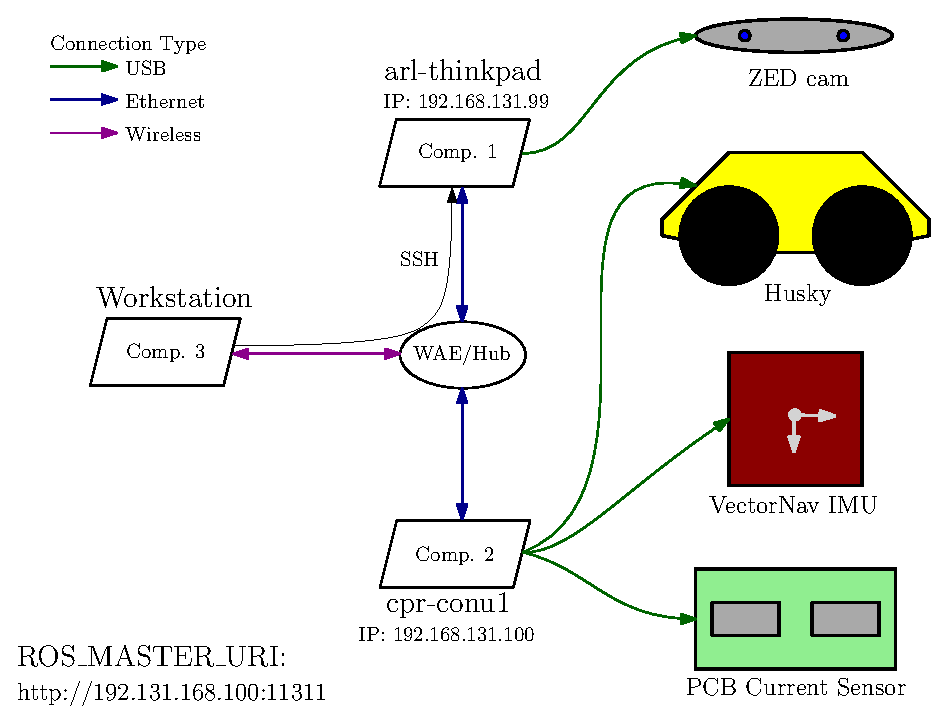
\includegraphics[scale=1]{figs/SetupOverview.eps}
	\caption{Overview of hardware Setup for 2020 field testing session. The workstation uses SSH to access \emph{arl-thinkpad}, where the \code{data\_collection} package is located. Sensor nodes and motion commands are launched from \emph{arl-thinkpad}, sending information over the network to \emph{cpr-conu1} when needed. Notice that although commands are sent from \emph{arl-thinkpad}, the Master URI is configured to be on \emph{cpr-conu1}; the reason for this is related to launch-on-boot features of the Husky and is discussed further in Section~\ref{sec:SoftwareConfiguration}.}
	\label{fig:SetupOverview}
\end{figure}

%----------------------------------------------------------------------------------------

\section{Network Configuration}
\label{sec:NetworkConfiguration}


To command the rover from the Main Computer, ensure that it is connected through a hub. For our experiments a Cisco Wireless Access Point/Hub was used.

\subsection{Usage}
\label{subsec:NetworkConfigurationUsage}

%----------------------------------------------------------------------------------------

\section{Software Configuration}
\label{sec:SoftwareConfiguration}

\subsection{Overview}

The field testing experiments are implemented using an array of different ROS packages, shell scripts, and devices; at the highest level these verious software items are localized and governed by the ROS package \code{data\_collection}. Code for the package is hosted at \url{https://github.com/brahste/data_collection}. The main access point to the hardware suite is through the file \code{husky\_sensors.launch}. Since Husky launches its nodes on boot-up (from the files in \code{/etc/ros/kinetic/}), \code{husky\_sensors.launch} is responsible for initializing the nodes for peripheral sensors only. A secondary consequence of the Husky nodes intializing on boot is that it is simplest to use \emph{cpr-conu1} as the Master URI (as shown in Fig.~\ref{fig:SetupOverview}). 

Although \emph{arl-thinkpad} hosts the main data collection package and the ZED node, packages for the IMU and motor current sensors had been configured for past field tests on \emph{cpr-conu1}; we have left this configuration intact. Since the Husky node initializes on boot, for this field testing session it was chosen to use \emph{cpr-conu1} as the Master URI. Future researchers may find it desirable to connect and configure all sensors to \textit{arl-thinkpad} and disable the launch-on-boot feature of Husky, this way the Master URI could be assigned to \textit{arl-thinkpad} and complications regarding network latency would be less pronounced.

Note that \code{husky\_sensors.launch} initializes nodes that exist on both \emph{arl-thinkpad} and \emph{cpr-conu1}. To enable this feature an environment configuration file \code{husky\_env.sh}, located in the main catkin workspace of \emph{cpr-conu1}, must be called when launching nodes over the network. 

\subsection{Cautionary statements}

Because of a ROS limitation the IMU launch file located on \emph{cpr-conu1} (which is called by \emph{arl-thinkpad}) has to be located at the same path on both machines. However, the file on \emph{arl-thinkpad} is merely symbolic as the rest of the \code{imu\_vn\_100} package is empty.

The IMU and terrain class publisher are linked at the same publication rate. This does not mean that their publications are synchronized; however, as the publication rate approaches zero, the time difference between publications will become negligible (like in calculus). The default rate is set to 200 Hz.

The bag files are recorded for the time is *should* take for the motion to execute. That is, the total distance commanded is calculated, and divided by the commanded velocity. It may be a good idea to add a few extra seconds on the end of this restriction such that some slip can be account for. In post processing a small threshold on the end of the IMU measurements can be used to truncate the data.

\subsection{Usage}

\begin{enumerate}
\item Before moving forward with this section, ensure the steps from Section~\ref{subsec:NetworkConfigurationUsage} are complete. Most importantly the \code{ROS\_MASTER\_URI}, hostnames, and IPs must be set correctly. At this point the Husky node should be running, this can be confirmed by calling \code{rosnode list}. If the nodes [...enter the names of a few nodes...] are up, then indeed the Husky node is running.
	
\item Initialize the peripheral sensors with: \\
  \code{roslaunch data\_collection husky\_sensors.launch}
  
  \qquad Running \code{rostopic list} you should now be able to see that \code{imu/rpy}, \code{imu/imu}, and \code{zed/*} are being published. As a sanity check (or for debugging) you can run \code{rostopic echo <topic\_name>} and see the data streams from each sensor in your terminal.

  It is important that the bagging be called and logged on \emph{arl-thinkpad} because

\end{enumerate}

Upon \code{roslaunch}-ing, the master node is initialized, along with the following nodes:

%\begin{enumerate}
%\item \verb zed_node  (confirm name of this node); this node is responsible for publishing sterero-image messages. 
%x\item \verb vectornav (confirm name of this node); this node is responsible for publishing messages from the IMU.
%\item \verb current_sensing  (confirm name of this node); this node is responsible for publishing message of current draw from the rover.
%\end{enumerate}

%Available image types and imaging parameters are outlined in Appendix~\ref{app:NodeInformation}.

\section{Running the Experiment}

Each experimental trial consists of a CLC-type path and a data logging procedure. Trials are initiated with \code{husky\_experiment.launch}; inside this file are relavent path specifiers, such as turning radius and linear segment travel distance. These path specifiers can be manipulated within the launch file by changing the default value, or by passing command line arguments. The former case is prudent when many of the specifiers are to be altered, while the latter is prudent for rapid experimental iteration over variations in a single (or few) specifiers. The data collected over the duration of each trial is saved in the \code{bags/} directory of \emph{arl-thinkpad}.

\begin{figure}
  \centering
  \includegraphics[width=0.6\textwidth]{figs/HuskyPanel.jpg}
\end{figure}

\subsection{Pre-experimental setup}
\begin{enumerate}
\item \textbf{Ensure the ZED cam is connected to \emph{arl-thinkpad}.} The connectivity of the ZED cam can be confirmed by ... [finish this section later].

\item \textbf{Ensure the IMU is connected to Husky's dedicated computer (\emph{cpr-conu1}).}

\item \textbf{Ensure both \emph{arl-thinkpad} and \emph{cpr-conu1} are connected via ethernet to the WAE/Hub and that the WAE/Hub is connected to power.} The ports that the computers are connected to are irrelevant, at the time of writing \emph{arl-thinkpad} was connected to Port 1 and \emph{cpr-conu1} was connected to Port 3.

\item \textbf{Ensure the Husky is either elevated with its wheels free (for in-lab testing), or you are in a large unobstructed area (for experimental testing).} Most importantly, \underline{do not} launch \code{husky\_experiment.launch} without precaution.
  
\end{enumerate}
  
\subsection{Starting the Experiment}
\begin{enumerate}
\item \textbf{Power on the Husky, \emph{cpr-conu1}, and \emph{arl-thinkpad}.} Because of Husky's launch-on-boot feature \code{roscore} will be initialized in the background.

\item \textbf{On \emph{arl-thinkpad} open a terminal}\footnote{This computer has been set up with terminator, a terminal emulator. Use Ctrl(Fn)+Shift+E and Ctrl(Fn)+Shift+O to split the terminal vertically and horizonatally.}. The environment has been automatically configured in the \code{.bashrc} file; you should see the ROS hostname, IP, and Master URI printed just above the command line.
  
\item (optional) \textbf{To verify connectivity you can access \emph{cpr-conu1} with,} \\
  \code{ssh administrator@cpr-conu1}. The SSH keys have already been configured so no password should be required; the ROS hostname, IP, and Master URI should also be shown just above the command line. Since the launch files depend on known SSH keys, if a password is prompted you may run into difficulties when running launch files in later steps. Either way, the password is: clearpath.

\item \textbf{Run} \code{\$ roslaunch data\_collection husky\_sensors.launch}. This command starts the various sensor nodes given the arguments in the executed launch file. It is worth the time so analyze the SUMMARY output to understand the values set on the parameter server and which nodes were initialized. An \code{rqt\_reconfigure} GUI will appear, here you can interact with the \\ \code{/terrain\_class\_publisher} value. It is recommended that parameters for the \code{/husky\_velocity\_controller} are left untouched.

\item (optional) \textbf{Verify topic publications with,} \code{rostopic echo <topic\_name>}.

\end{enumerate}
 
\subsection{Running Experimental Trials}

\begin{enumerate}

\item \textbf{As a first test, run} \code{\$ roslaunch data\_collection husky\_experiment.launch}. This will start the Husky moving along the default path. You should be able to see the port-side wheels turning faster than the starboard-side. A \code{.bag} file will be saved in the \code{bag/} directory with all trial parameters. Since the algorithm depends on IMU inputs to know when it is has reached the selected yaw, if this command is run when the Husky is elevated, you will have to Ctrl+C out of the program. With default parameters it will take approximately 30 seconds for the published topics to be bagged.

\end{enumerate}


\cleardoublepage
\appendix

\section{Operating System Configuration}
\label{app:OperatingSystemConfiguration}

\section{Node Information}
\label{app:NodeInformation}


\end{document}
